\documentclass[a4paper,12pt]{report} 
\usepackage[utf8]{inputenc}
\usepackage[T1]{fontenc}
\usepackage[margin=2.5cm]{geometry}
\usepackage[parfill]{parskip}
\usepackage{url}
\usepackage[nottoc,numbib]{tocbibind}
\usepackage[pdftex]{graphicx}


\newcommand*{\TitleFont}{%
  \usefont{\encodingdefault}{\rmdefault}{b}{n}%
  \fontsize{24.88}{50}%
  \selectfont}

\newcommand*{\TitleFontTwo}{%
  \usefont{\encodingdefault}{\rmdefault}{b}{n}%
  \fontsize{20.74}{20}%
  \selectfont}

\renewcommand\bibname{References}


\title{\TitleFontTwo DD2476: ir13 \\ \TitleFont Reputation Estimation using Twitter}


\author{Ludwig Forsberg \\ \hspace{0.5cm} \small\texttt{ludwigf@kth.se} \hspace{0.5cm} \and Romain Pomier \\ \small\texttt{romain.pomier@gmail.com} \and Kristoffer Hallqvist \\ \small\texttt{khallq@kth.se} \and Thibaut Patel \\ \small\texttt{thibaut.patel@gmail.com}}

\begin{document}

\maketitle
\clearpage

\abstract{
In this report we explore the possibility of measuring the opinion of a group of people using messages from twitter. At first we give a short introduction to the rationale of trying to analyze communication in order to extract the opinion. Then we explain why communication over twitter was used as well as exactly how the analysis, and the evaluation of the analysis, would be made. We used lexicons, Support Vector Machines and our own ``influence algorithm'' in order to perform the analysis and then we manually classified some tweets and made use of polls in order to evaluate our analysis. We explain how these components was used to both construct and evaluate our analysis, then we present the result that we got. Finally we discuss the results, present ideas of measures that could be made to improve them and some conclusions that could be made. At best we got a 58\% accuracy when it comes to classifying the tweets, and the analysis yielded a value that was a x percents off the poll whereas simply counting tweets was y percents off.
}

\clearpage
\thispagestyle{empty}
\vspace*{2.15cm}
\title{\huge \textbf{Statement of collaboration}}
\vspace{1cm}\\
\title{\large \textbf{Ludwig Forsberg}}
\begin{itemize}
    \item Implemented 6/7 of the lexicons as well as the program that combines separate lexicons into one lexicon
    \item Implemented some of the program that uses all of the different components to yield a result
    \item Implemented the tool to perform the manual classification
    \item Wrote the Introduction
    \item Wrote the Method, Lexicon, Manual and Poll part in the Method section
    \item Wrote about 1/3 of the Discussion and Conclusion section
    \item Wrote the Introduction and Method sections of the Poster
\end{itemize}
\title{\large \textbf{Romain Pomier}}
\begin{itemize}
  \item Pre-processing of words given to the lexicons and the SVM
  \item Use of the SVM (features extraction, learning, classification)
  \item Writing of the scripts that perform the tests
\end{itemize}
\title{\large \textbf{Kristoffer Hallqvist}}
\begin{itemize}
  \item item1
  \item item2
  \item item3
\end{itemize}
\title{\large \textbf{Thibaut Patel}}
\begin{itemize}
  \item item1
  \item item2
  \item item3
\end{itemize}


\tableofcontents

\clearpage
\chapter{Introduction}

\section{Background}

There has always been a desire to read people's minds.
To extract the will of the people, to be able to find the best movie, adapt ones business strategy to better appeal to ones customers or for more sinister purposes such as trying to control ones inhabitants by an authoritarian government.

To directly read someones more advanced thoughts is however still far from possible.
However how and what a person chooses to communicate do very often reflect what the person thinks.
The sheer volume of communication that occurs today is however so great that attempting to have actual people analyzing it is infeasible. 
The only entity with the amount of processing power required are computers. 
To analyze a text-message in order to extract the thoughts of the sender is however a very daunting task for a computer, even a human that has trained and evolved tools designed to achieve this feat over thousands of years has difficulties.

In computer science the problem of extracting subjective information in source materials is called sentiment analysis or opinion mining. 
The most basic task in this field is usually to simply classify the polarity of a text, i.e. if it is positive or negative. 
This is sometimes called semantic orientation. 

The focus of the bulk of the research on automated text-analysis has rested on trying to classify separate texts.

\section{Problem Description}

In our project we are interested in examining how the classification of text in tweets passed between people in a population actually corresponds with the populations opinion of a particular brand and explore if utilizing the number of followers, retweets and favorites, something we call ``reach'', of a tweet would better capture the opinion of the population then just using a classification of the texts. 

\chapter{Method}

To try to keep it simple we decided to estimate where in a range between negative and positive the opinion of the people would be of a particular brand.
However in order to utilize the reach of a tweet we first need to at least determine if the message itself is negative or positive, or where in the range it is.
So we are forced to first do a classification using only the text to be able to use the algorithm.

To perform this text-based classification we chose to use a Support Vector Machine (SVM) because that approach appeared to get the best results when comparing results from \cite{Pang02} and \cite{Turney02}.
We also decided to use a supervised approach which means that we provide the SVM with messages that already had been classified to train on.
To get these classified messages we decided to use lexicons to classify all the messages and then pick a number of the messages with the highest ranking in each category for the SVM to train on.

To make sure the results from the lexicons and the SVM were reasonable we considered it necessary to evaluate them as well. 
In order to do this we manually classified a number of tweets and then used the lexicon and the SVM to classify those same tweets as well and compared the results.

Once the SVM had made the initial classification on the text we translated it to a position in the range between negative and positive, then we applied our algorithm and received another position. Finally to evaluate both of these positions we decided to use a poll on the subject that had yielded a position on a similar range.

To be able to use good polls, and get a lot of relevant tweets to process, we decided to evaluate our analysis on three different well-known brands; Disney, Costco and Coca Cola.

\section{Crawler}

As we need a considerable amount of data to train and test our algorithm, we need a dataset of tweets. Given that we are also using the meta information of the tweets (number of retweet for example), we could not find preexisting datasets and we chose to directly harvest Twitter.
We use the Twitter search as an entry point in the Twitter flow of data. This enables us to get pertinent information by getting only the tweets containing the name of brands we choose.

We have observed in the different research papers that after getting the raw information, there is a filtering step. We chose not to do this part ourselves. In order to reduce the scope of the project, we only consider the English language. This filtering is done at the harvesting time by using the Twitter language filter.
We also assume that there is no topic drift in a tweet. That is to say if the tweet contains the name of the brand, its content is going to be about this brand.

The quantity of information extracted from Twitter corresponds to the maximum amount of tweets we can get from a search at a given time : Twitter index only the tweets from the last 6 to 9 days.

For the 3 brands chosen, Coca Cola, Costco and Disney, we got respectively 4592, 7164 and 7403 tweets, with the selected metadata that is used in our algorithm.

\section{Lexicon}

We used seven different lexicons one containing about 200 unique words, five containing about 900 unique words and one containing about 7000 unique words.
One of the lexicons consisted of simply two lists of negative and positive words where the rest listed words with a certain negative and positive score between 0 and 1. 
Some of these lexicons had support for an NLP approach where some words had different scores if they were present in a text as an adjective or an adverb.  
But to ease the aggregation of the different lexicons we choose to keep it simple and just considered the probability of a word being adjective or adverb to be equal for example.

The lexicons were used in simple bag-of-words model of the text so each word was sent to all lexicons, scored with a value between 0 and 1 in both negativity and positivity and then returned. 
The score of a tweet was then created by summing up the score for all the words in all the lexicons.

We performed a pre-processing of the words using the \textit{Natural Language Toolkit} python plugin.\cite{NLTK}.
We remove the punctuation, then we use a stemmer and lemmatizer, thus for instance we transform all variations "loving", "loves" and "loved" into simply "love".
That makes it easier for the lexicon to recognize words.

\section{SVM}

We used a Support Vector Machine (SVM) to get the polarity of a tweet. It is a supervised learning model that recognize patterns. We used the python plugin \textit{scikit-learn}\cite{Scikit} and its implementation of the SVM to make it work.

Our goal is to create a SVM specialized in one company, because we believe that a word witch is polarized for one company don't have to be polarized for another.
For instance, the word \textit{sample} is positive when talking about CostCo because they offer a lot of samples and people seems to enjoy it. However, a \textit{sample} when talking about Disney would probably be a sample of a movie, and then should be neutral.
That is the king of informations our SVM is supposed to extract.

First we had to make our SVM learn. To that purpose we used our lexicon to create training data. Among all the tweets about a company, we label as "positives" the $n$ tweets with the highest positive score given by the lexicons. Likewise, we label as "negatives" the $n$ tweets with the highest negative score. Finally, we label as "neutral" the $n$ longest tweets which have both null positive and negative score. The SVM will then learn from these $3n$ tweets.

To represent a tweet, we chose as features its unigrams and bigrams. We use the same pre-processing of words than with the lexicons.

Finally, to guess the polarity of a random tweet about the company, we extract its features, and then classify it thanks to the SVM.

\section{Tweaks}

Thanks to the previous parts, we are now in possession of the tweets associated with their polarity (positive, negative or neutral). Our goal is to extract global information from this new dataset.
This is the novelty aspect in our work, and we chose to present two ways of grouping this polarity information.

What we aim for is a measure for the popularity of a brand. It is achieved by aggregating the polarity of each tweet, weighted by their influence over the network.
Then the main aspect of our work consists in finding the right way to measure the influence of a tweet.

The influence measure is critic. It is the measure that enables us to aggregate the polarity of a tweet in order to get an overall opinion on a brand.

Thanks to this measure, we can extract a first statistic : the top 10 influencial tweets. This is a simple extraction given the influence score of each tweet, but this is increasing the actionability of our results, which means that a company using this results can take action by contacting the author of those tweets for example.

The overall opinion score is our main goal, and once we have computed the polarity and the influence of each tweet, we sum the influence of the positive tweets and divide this result by the sum of the influence of the positive and negative tweets.

\section{Manual}

To manually score tweets we made a little script that asked the user what file the user wants to process. 
Then the user is presented with a text and asked to classify it where the options are positive, positive but unsure, negative, negative but unsure, neutral and neutral but unsure. 
The user is free to go back and re-classify a tweet but cannot pass a tweet, to classify new tweets the last tweet presented must be classified. 
Once a number of tweets has been classified the user can save his progress in a separate file and quit. 
When the user resumes the classification process the classification will also resume where he left off.

\section{Poll}

In order to compare our results to something that measured the actual opinion of the people we decided that we more or less needed some kind of poll. 
Polls are far from perfect but should be accurate enough for our purposes. It was quite difficult to find a poll that measured the general opinion of a company. 
Most polling institutes are hesitant to disclose their raw data and instead they present their own trademarked metrics that are usually an aggregation of a wide array of different parameters.

We did however find a poll by Harris Interactive made quite recently (November 13-30 in 2012) that had quite a large numbers of interviews (14 000) \cite{Harris13}. 
It also contained a section where they had a category called “Emotional Appeal” that was an aggregation of answers to how much the interviewee “Feel good about”, “Admire and Respect” and “Trust” the brand in question on a 0-7 range. 
These three scores were then summed up, divided by 21 and multiplied by 100 in order to essentially create a general score for the emotional appeal for the brand \cite{Harris13}. 
We felt this would correspond to the opinion of the population accurate enough for our purposes.

\chapter{Results}

\section{Manual classification}

These are the results of the manual classification of the first 100 tweets for each brand. Each member of the group individually classified the tweets, and these are the average polarities for the different brands.

\centerline{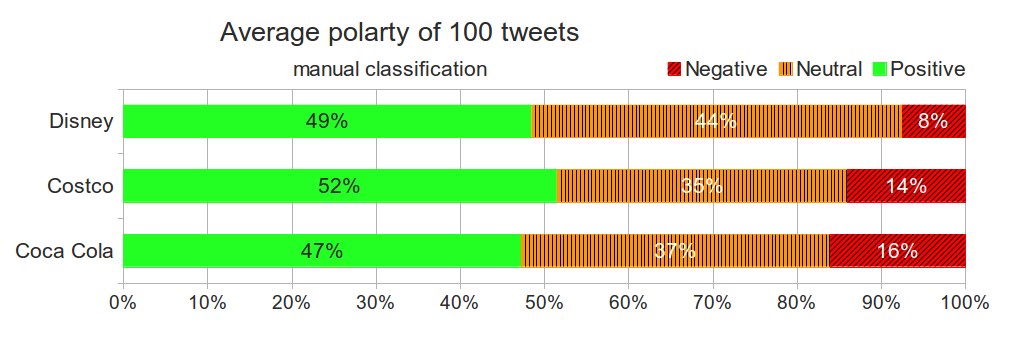
\includegraphics[scale=0.6]{../img/man1.png}}

The fact that we classified them individually led to quite a few disagreements:

\begin{itemize}
        \item \textbf{Coca Cola}: All of us agreed on 42\% of the tweets.
        \item \textbf{CostCo}: All of us agreed on 51\% of the tweets.
        \item \textbf{Disney}: All of us agreed on 34\% of the tweets.
\end{itemize}

For example, this means that out of the 100 Coca cola tweets, there were 42 which we all classified according to the same polarity, and 58 where at least one member disagreed with the others.

\section{Lexicon evaluation}

Using the results of our manual classification on tweets about Coca Cola, Disney and CostCo, we were able to evaluate the results of our unsupervised classification with the lexicon score on these three companies.
To classify a tweet with the lexicon, we get the positive and the negative score of this tweet, subtract one to the other, and finally apply an arbitrary threshold to get the classification.
This threshold was set to 2, so that if the score is greater than 2 the tweet is classified as positive, if the score is less than -2 the tweet is negative, and otherwise to tweet is classified neutral.

Here are the results we got on the 100 tweets we classified manually for each company:
\begin{itemize}
        \item \textbf{Coca Cola}: the lexicon agrees on 53\% of the tweets.
        \item \textbf{CostCo}: the lexicon agrees on 58\% of the tweets.
        \item \textbf{Disney}: the lexicon agrees on 58\% of the tweets.
\end{itemize}
Looking more deeply on the results, we can see that our lexicon method doesn't take a lot of risks.
Most of the mistakes consist in classifying as neutral a positive or negative tweet. That means it is unable to detect any sentimental parts in theses tweets, because they are too short, too ironic, or because the sentimental part is actually contained in the emoticons or hashtags.\\
For instance, the following tweets are classified as neutrals, while they are actually positives:\\
\centerline{\textit{Costco Sundays!!}}\\
\centerline{\textit{Need to do a Costco run today... :) \#LoveThatStore}}

\section{SVM classification}

Using the results  of our manual classification once again, we have also evaluated our SVM classifier.
We used 450 tweets to make the SVM learn, based on the method previously described.

Here are the results we got on the 100 tweets we classified manually for each company:
\begin{itemize}
        \item \textbf{Coca Cola}: the SVM agrees on 48\% of the tweets.
        \item \textbf{CostCo}: the lexicon agrees on 50\% of the tweets.
        \item \textbf{Disney}: the lexicon agrees on 16\% of the tweets.
\end{itemize}
We can see that the results are below the ones we got with the lexicon method.
That means that our SVM was not able to remove the noise in the learning data induced by the lexicon method.\\
In the case of Coca Cola and CostCo, results are pretty close to the previous ones, with around 50\% of matching.
For Disney however, results are really bad. Our guess is that as Disney has more diversified activities than the two other companies (movies, tv, amusement park, ...), the topics talked about are really different, thus the SVM would need a lot more learning datas to classify tweets correctly.

Looking closer to the results, we can see that unlike with the lexicon method, this method doesn't tend to classify as neutral when it makes mistakes.
It often classifies a negative tweet as positive and vice versa.
That means that its mistakes are more serious.






\chapter{Discussion/Conclusion}
Tweets are notoriously difficult to classify. Due to the small character limitations (140 characters) people often utilize the context to a high degree in their messages which even makes classification for humans difficult if the messages are stripped of their context. Computers can not utilize the context to the same degree as humans but they suffer from this fact as well. One positive effect of the small character limitation with respect to classification is that tweets often only contain one semantic orientation about one particular thing.

This results from classification using only lexicons was about 50\% accurate when compared to the manually classified tweets wich is good but far from great. To improve this results one may simply acquire more lexicons and use more sophisticated POS tagging. 

Six out of the seven lexicons we did use came from the same source. Those six were created by applying six different machine-learning techniques on the same initial corpus. That may have led to some issues such as giving too much importance to some words only because they were present in this initial dictionary.

We may also improve our usage of the lexicons. At the moment we don't use a Part-Of-Speech tagging, so the polarity of a word is evaluated regardless of the context of the word. For example "very good" and "not very good" will more or less yield the same result. It would be good also to consider the position of the company name, so that we can see the difference between "Costco is great but I dislike ice-cream" and "I dislike Costco but I think ice-cream is great".

The results from using the Support Vector Machine are pretty poor. We suspect two main reasons for this.

First, using unigrams and bigrams as features may not be enough. To get better results, we should add more relevant features, like for example information about the urls (number, domain name, …), about the emoticons (number of positives, negatives) or about the tweet as a whole (length, number of verbs, number of adjectives etc).

Second, we trained our SVM with data that contains a lot of noise when we used the output of the lexicon to generate training data. The lexicon method offered a 50\% match on our manually classified, which doesn’t look good enough for learning purpose.

The poll that was used was an aggregation of rankings done on three different subjects (“Feel good about”, “Admire and Respect” and “Trust”). The value for these should be quite strongly correlated among themselves and also to the fact that they people who were interviewed actually “like” or “dislike” a brand. But we have no real scientific way of knowing.

We do know that the survey we used was exclusively performed in America. Unfortunately there is no way to filter tweets on the origin but one could at least filter it on language. To filter on english unfortunately does not exclude all non-americans (since it is such a global language). To make sure that the poll used is made on the same people that make the tweets one could use a poll conducted on people with a very local language and then filter on that language. The poll was conducted quite recently however.

Concerning the limitation of the influence computation, we couldn't find any existing result to compare the efficiency of our formula. However the resulting computation comes from tries and error when applying the function to our dataset, and seems to give good results. More research can be done in this part of our study in order to bring a deeper analysis of our results.

We are really interested in developing the actionability of our solution, that is to say that a company using our solution could take action according to the result of the program’s computation. There is several tweaks that could have been applied to our solution in order to offer a wider range of tools for a company.

As we implemented the top 10 influential tweets, we wanted to continue in the same direction by implementing the top influential Twitter users. This features enable the company to get a better reach on its customers by using these influential intermediaries. We would have used a similar “influential weight” that what we use for the influential tweets, but aggregating this measure by author.

Another extension to the current solution would be to work with the links embedded in tweets. The first step would be to rank the top articles, and to crawl their title, in order to present an understandable list of articles that were shared and read by a lot of the consumers. We also had the idea of taking this reputation management further by computing the polarity of the article. We would then extend our reputation management to the pages linked from Twitter, which would give a much broader coverage, even if I would need new tools to analyze the polarity of an article because of the different nature of an article versus a tweet.

In the end we conclude that our results are far from perfect but that they hint at the fact that using parameters such as followers, retweets and favorites do improve the estimation of the opinion of a population over simply trying to calculate the opinion of separate tweets and then summing up the amount of tweets of each opinion.

To get a definitive answer on this matter one would have to get much better results using the lexicons and SVM in a much more sophisticated way.

\begin{thebibliography}{9}

%These references are very flexible to make however you want them, if you want them in a different format I'm open to suggestions
  
\bibitem{Pang02}
  Bo Pang, Lillian Lee and Shivakumar Vaithyanathan\\
  \emph{Thumbs up? Sentiment classification using machine learning techniques} (2002)\\
  \url{http://www.cs.cornell.edu/home/llee/papers/sentiment.pdf} (2013/05/14)

\bibitem{Turney02}
  Peter Turney\\
  \emph{Thumbs Up or Thumbs Down? Semantic Orientation Applied to Unsupervised Classification of Reviews} (2002)\\
  \url{http://arxiv.org/pdf/cs/0212032v1} (2013/05/14)
  
\bibitem{NLTK}
  Natural Language Toolkit, a python plugin. Website:\\
  \url{http://nltk.org/}
  
\bibitem{Scikit}
  Scikit python plugin website:\\
  \url{http://scikit-learn.org/stable/}

\bibitem{Harris13}
  Harris Interactive\\
  \emph{The Harris Poll 2013 RQ® Summary Report} (2013)\\
  \url{http://www.harrisinteractive.com/vault/2013 RQ Summary Report FINAL.pdf} (2013/05/15)

\end{thebibliography}


\end{document}
